\chapter{Forces and Momentum}
\section{Force and Motion}
The previous two sections of this module have focussed on kinematics, or how things move, now we turn to \textbf{dynamics}, or why objects move.  Forces are responsible for why objects move. Think of pushing someone on a swing, if you did not give them the initial push they would not start moving. Or think of gravity pulling down on an object, if I let go of an apple it will fall. If an object, or system of objects, changes the state of another, it does so by applying a force. The obvious everyday examples are things that \textbf{push} and \textbf{pull}. \\

Some forces like friction require contact between the objects to act, we call these \textbf{contact forces}. Think of rolling a ball across a table, does it matter what the table is made of? Yes, the rougher the table is the higher its friction and the faster the ball will come to a stop. Other forces, e.g. gravity, magnetism, \dots{}, act over a distance. These are called either \textbf{long range} or \textbf{short range} forces, depending on how long a distance they can act over. \\

Forces are vectors as they have both a magnitude, how strong the effect of the force is, and a direction, which direction the force wants the object to move in.  Since we can have more than one force acting on an object we understand them using a free body diagram as in \cref{fig: free body diagram}. The motion of the object will be governed by the net force, the vector sum, of all the forces acting on the object. This net force is often called the \textbf{resultant}, and the process of finding it is referred to as \textbf{resolving} the forces on the object.\\

Typically when there are more is more than one force acting on an object we use a \textbf{free body diagram} to help us understand the situation. An example free body diagram for an object hanging on the end of a piece of string is given in \cref{fig: free body diagram}.  A free body diagram is not a detailed scale drawing of the problem, it is a diagram depicting a simplified version of the body, all the forces acting on the object as arrows pointing in the direction that they are acting. When solving a problem involving forces it is often a good idea to start with a free body diagram so that you can work out what the net force is.

\begin{center}
\begin{figure}[ht]
\ThisAltText{ A free body diagram showing the forces acting on an object of mass m suspended from a string.}
\def\iangle{35} % Angle of the inclined plane
\def\down{-90}
\def\arcr{0.5cm} % Radius of the arc used to indicate angles
    %\centering
   % \pdftooltip{
   \begin{tikzpicture}[
    force/.style={>=latex,draw=blue,fill=blue},
    axis/.style={densely dashed,gray,font=\small},
    M/.style={rectangle,draw,fill=white,minimum size=0.5cm,thin},
    m/.style={rectangle,draw=black,fill=white,minimum size=0.3cm,thin},
    plane/.style={draw=black,fill=blue!10},
    string/.style={draw=red, thick},
    pulley/.style={thick},]
\node[m] (m) {$m$};
    \draw[axis,->] (m) -- ++(0,2) node[left] {$+$};
    {[force,->]
        \draw (m.north) -- ++(0,1) node[right] {$T$};
        \draw (m.south) -- ++(0,-1) node[right] {$W=mg$};
    };
\end{tikzpicture}
%}{A free body diagram showing the forces acting on an object of mass m.}
    \caption{A free body diagram showing the forces acting on an object of mass $m$ suspended on a string. The weight of the object is pointing down and is given by $W=mg$, and the tension in the string is pointing upwards and is $T$. }
    \label{fig: free body diagram}
\end{figure}
\end{center}

\paragraph{Example 4.1:} Consider an object of weight $\vec{W}$ on an inclined plane, with angle $\theta$. There are three forces acting on the object:
\begin{itemize}
\setlength{\itemsep}{-5pt}
    \item Gravity acts on the objects centre of mass and points straight down to the surface of the Earth. This gives rise to the objects weight $W$.
    \item The object does not fall through the plane due to the support force $S$ acting perpendicular to the plane.
    \item The friction of the plane $F_{r}$ acts on the object, this points upwards along the plane as it is what stops the object from sliding down the plane.
\end{itemize} 

\begin{figure}[ht]
    \centering
   % \pdftooltip{
   \ThisAltText{A picture of a mass on an inclined plane.}
   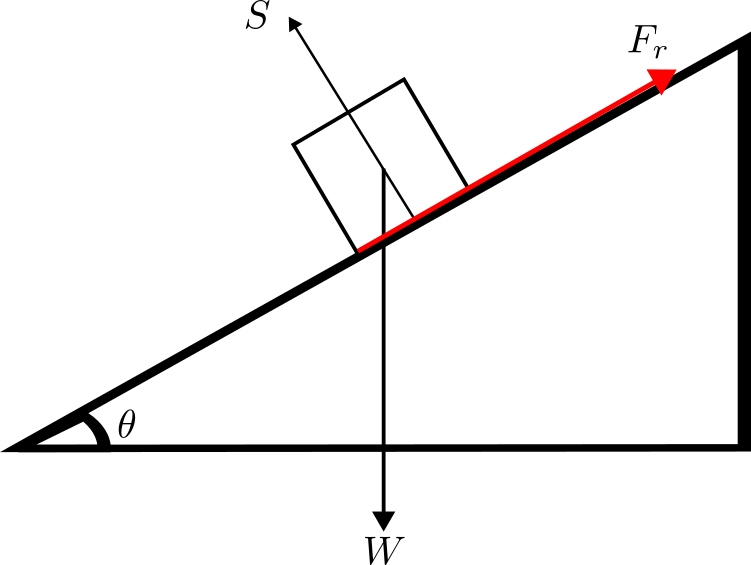
\includegraphics[width=0.4\textwidth]{figures/inclined_plane.png}
   %}{An inclined plane with a mass on it.}
    \caption{An inclined plane with a mass on it. The massive block has three forces acting on it, $W$ its weight pointing straight down, the support force of the plane $S$ acting perpendicular to the plane, and friction $F_{r}$. If this was a free body diagram we would not show the plane and just depict the mass with forces acting on it and the angles that they act at.}
\end{figure}

To understand if the object will move or not we need to resolve the forces and find if there is a net force acting in any direction. If the forces \textbf{balance}\footnote{Here balance means that the resultant vanishes $\vec{W}+\vec{S}+\vec{F}_{r}=\vec{R}=0$.} then the object will be stationary, if they do not balance then the object will slide down the slope. \\


\textbf{Question:} Do you think that whether the object slides down or not depends on the mass of the object or just on the angle of the slope?\\


When the net force $\vec{F}_{\text{net}}$ acting on an object vanishes we say that the object is in \textbf{equilibrium}. Often there is a lot of trigonometry involved in resolving forces so it is a good idea to get a lot of practice doing it.\\

A very common force that we interact with every day is gravity. It acts to attract mass to the centre of the Earth and is responsible for the weight\footnote{Remember that mass and weight are not the same, mass is a scalar quantity that measures the amount of stuff making up an object, while weight is the force of gravity acting on that mass. If you went to the moon where gravity is weaker your mass would be the same but your weight would have decreased.} of an object. For an object of mass $m$, measured in kg, its weight is give by
\begin{equation}
W=mg,
\end{equation}
where $g=-9.8\text{m/s}^{2}$ is the acceleration due to gravity. Remember that the negative sign is there to signify that gravity points downwards. The unit of force is known as the Newton and has the symbol N. \\


To understand how to resolve forces it is best to consider the following example.
\paragraph{Example 4.2:} Consider a $10$kg mass suspended from two pieces of string at angles $70^{\circ}$ and $30^{\circ}$ respectively.  What is the tensions in the strings so that the mass hangs at equilibrium.
\begin{figure}[ht]
    \centering
    %\pdftooltip{
    \ThisAltText{ A mass hanging from two strings at specified angles from the horizontal.}
    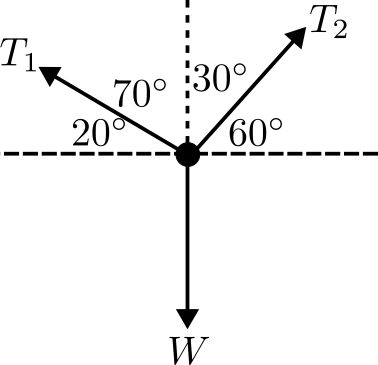
\includegraphics[width=0.3\textwidth]{figures/hanging_mass.png}
    %}{a hanging mass attached to two wires}
    \caption{A $10$ kg mass hanging from two wires.}
    \label{fig: hanging mass}
\end{figure}
\textbf{Tension} is the name for the force in the string pulling the mass upwards, it points along the string.  To understand this problem we can either add together the forces as vectors, or work component wise. In either case, we need to understand the horizontal and vertical components of the vectors.\\

This is easiest for the weight since it only points vertically so the horizontal component vanishes, $W_{x}=0$, and $W_{y}=W$. For the tensions we need to evaluate the components. The angles that we have been given are the angles between the string and the vertical, while we can work with these it is easier to work with the angle between the strings and the horizontal, these are depicted in \cref{fig: hanging mass} as the angles under the string.

\begin{figure}[ht]
    \centering
    %\pdftooltip{
    \ThisAltText{ A triangle showing how to decompose a force into its horizontal and vertical components.}
    \begin{tikzpicture}[scale=2]
  \coordinate [label=left:$60^{\circ}$] (C) at (-1.5cm,-1.cm);
  \coordinate (A) at (1.5cm,-1.0cm);
  \coordinate (B) at (1.5cm,1.0cm);
  \draw (C) -- node[above] {$T_{2}$} (B) -- node[right] {$T_{2y}$} (A) -- node[below] {$T_{2x}$} (C);
  \draw (1.25cm,-1.0cm) rectangle (1.5cm,-0.75cm);
  \tkzMarkAngle[size=1cm,color=blue](A,C,B)
 % \tkzMarkAngle[size=1cm,color=blue](C,B,A)
\end{tikzpicture}
%}{The components of the tension T2.}
    \caption{The components of the tension $T_{2}$.}
    \label{fig: Tension components}
\end{figure}

For $T_{2}$ the horizontal and vertical components are:
\begin{align*}
T_{2x}&=T_{2}\cos(60^{\circ}),\\
T_{2y}&=T_{2}\sin(60^{\circ}).
\end{align*}
Similarly for $T_{1}$ we have:
\begin{align*}
T_{1x}&=-T_{1}\cos(20^{\circ}),\\
T_{1y}&=T_{1}\sin(20^{\circ}),
\end{align*}
where the sign in $T_{1x}$ is there to show that it points to the left.\\

We know that at equilibrium the net force, $F_{\text{net}~}=W+T_{1}+T_{2}$ must vanish, this means that both its horizontal and vertical component must vanish. In other words:
\begin{align}
0&=W+T_{1y}+T_{2y}=W +T_{1}\sin(20^{\circ})+T_{2}\sin(60^{\circ}) \label{eq: vertical force components},\\
0&=T_{1x}+T_{2x}= T_{2}\cos(60^{\circ}) -T_{1}\cos(20^{\circ}) \label{eq: horizontal force components}.
\end{align}
This is a system of equations that we can solve for $T_{1}$ and $T_{2}$. The second equation tells us that 
\begin{align*}
T_{2}=T_{1}\frac{\cos(20^{\circ})}{\cos(60^{\circ})},
\end{align*}
substituting this into the first gives
\begin{align*}
-W=-mg	&=T_{1}\sin(20^{\circ})+T_{2}\sin(60^{\circ})\\
		&=T_{1}\sin(20^{\circ})+T_{1}\frac{\cos(20^{\circ})}{\cos(60^{\circ})}\sin(60^{\circ})\\
		&=T_{1}\left(\sin(20^{\circ})+\frac{\cos(20^{\circ})}{\cos(60^{\circ})}\sin(60^{\circ})\right).
\end{align*}
Now use that $-W=-mg=-10\times (-9.8)=98\text{N}$ and evaluate the trig functions to find:
\begin{align*}
98&=T_{1}\left(0.342+0.866\times\frac{0.9397}{0.5}\right)=1.97T_{1},\\
\Rightarrow T_{1}&=49.8\text{N},\\
T_{2}&=T_{1}\frac{\cos(20^{\circ})}{\cos(60^{\circ})}=49.8\times \frac{0.9397}{0.5}=93.5\text{N}
\end{align*}

Thus the tension in the strings are $T_{1}=49.8$ N and $T_{2}=93.5$N respectively, notice that here we are giving the magnitude of the vector hence both results are positive.\\

There are further examples of resolving forces given in the tutorial problems.

\section{Newton's Laws}
\textbf{Newton's laws}, sometimes referred to as Newton's laws of motion, describe how forces are related to the motion of objects. When you first encounter them they can seem counter intuitive, but they have been very well validated through experiments. There are three laws with each telling us something about how forces cause objects to move.

\begin{figure}[ht]
    \centering
    %\pdftooltip{
    \ThisAltText{ A picture of Sir Isaac Newton from Wikimedia commons.}
    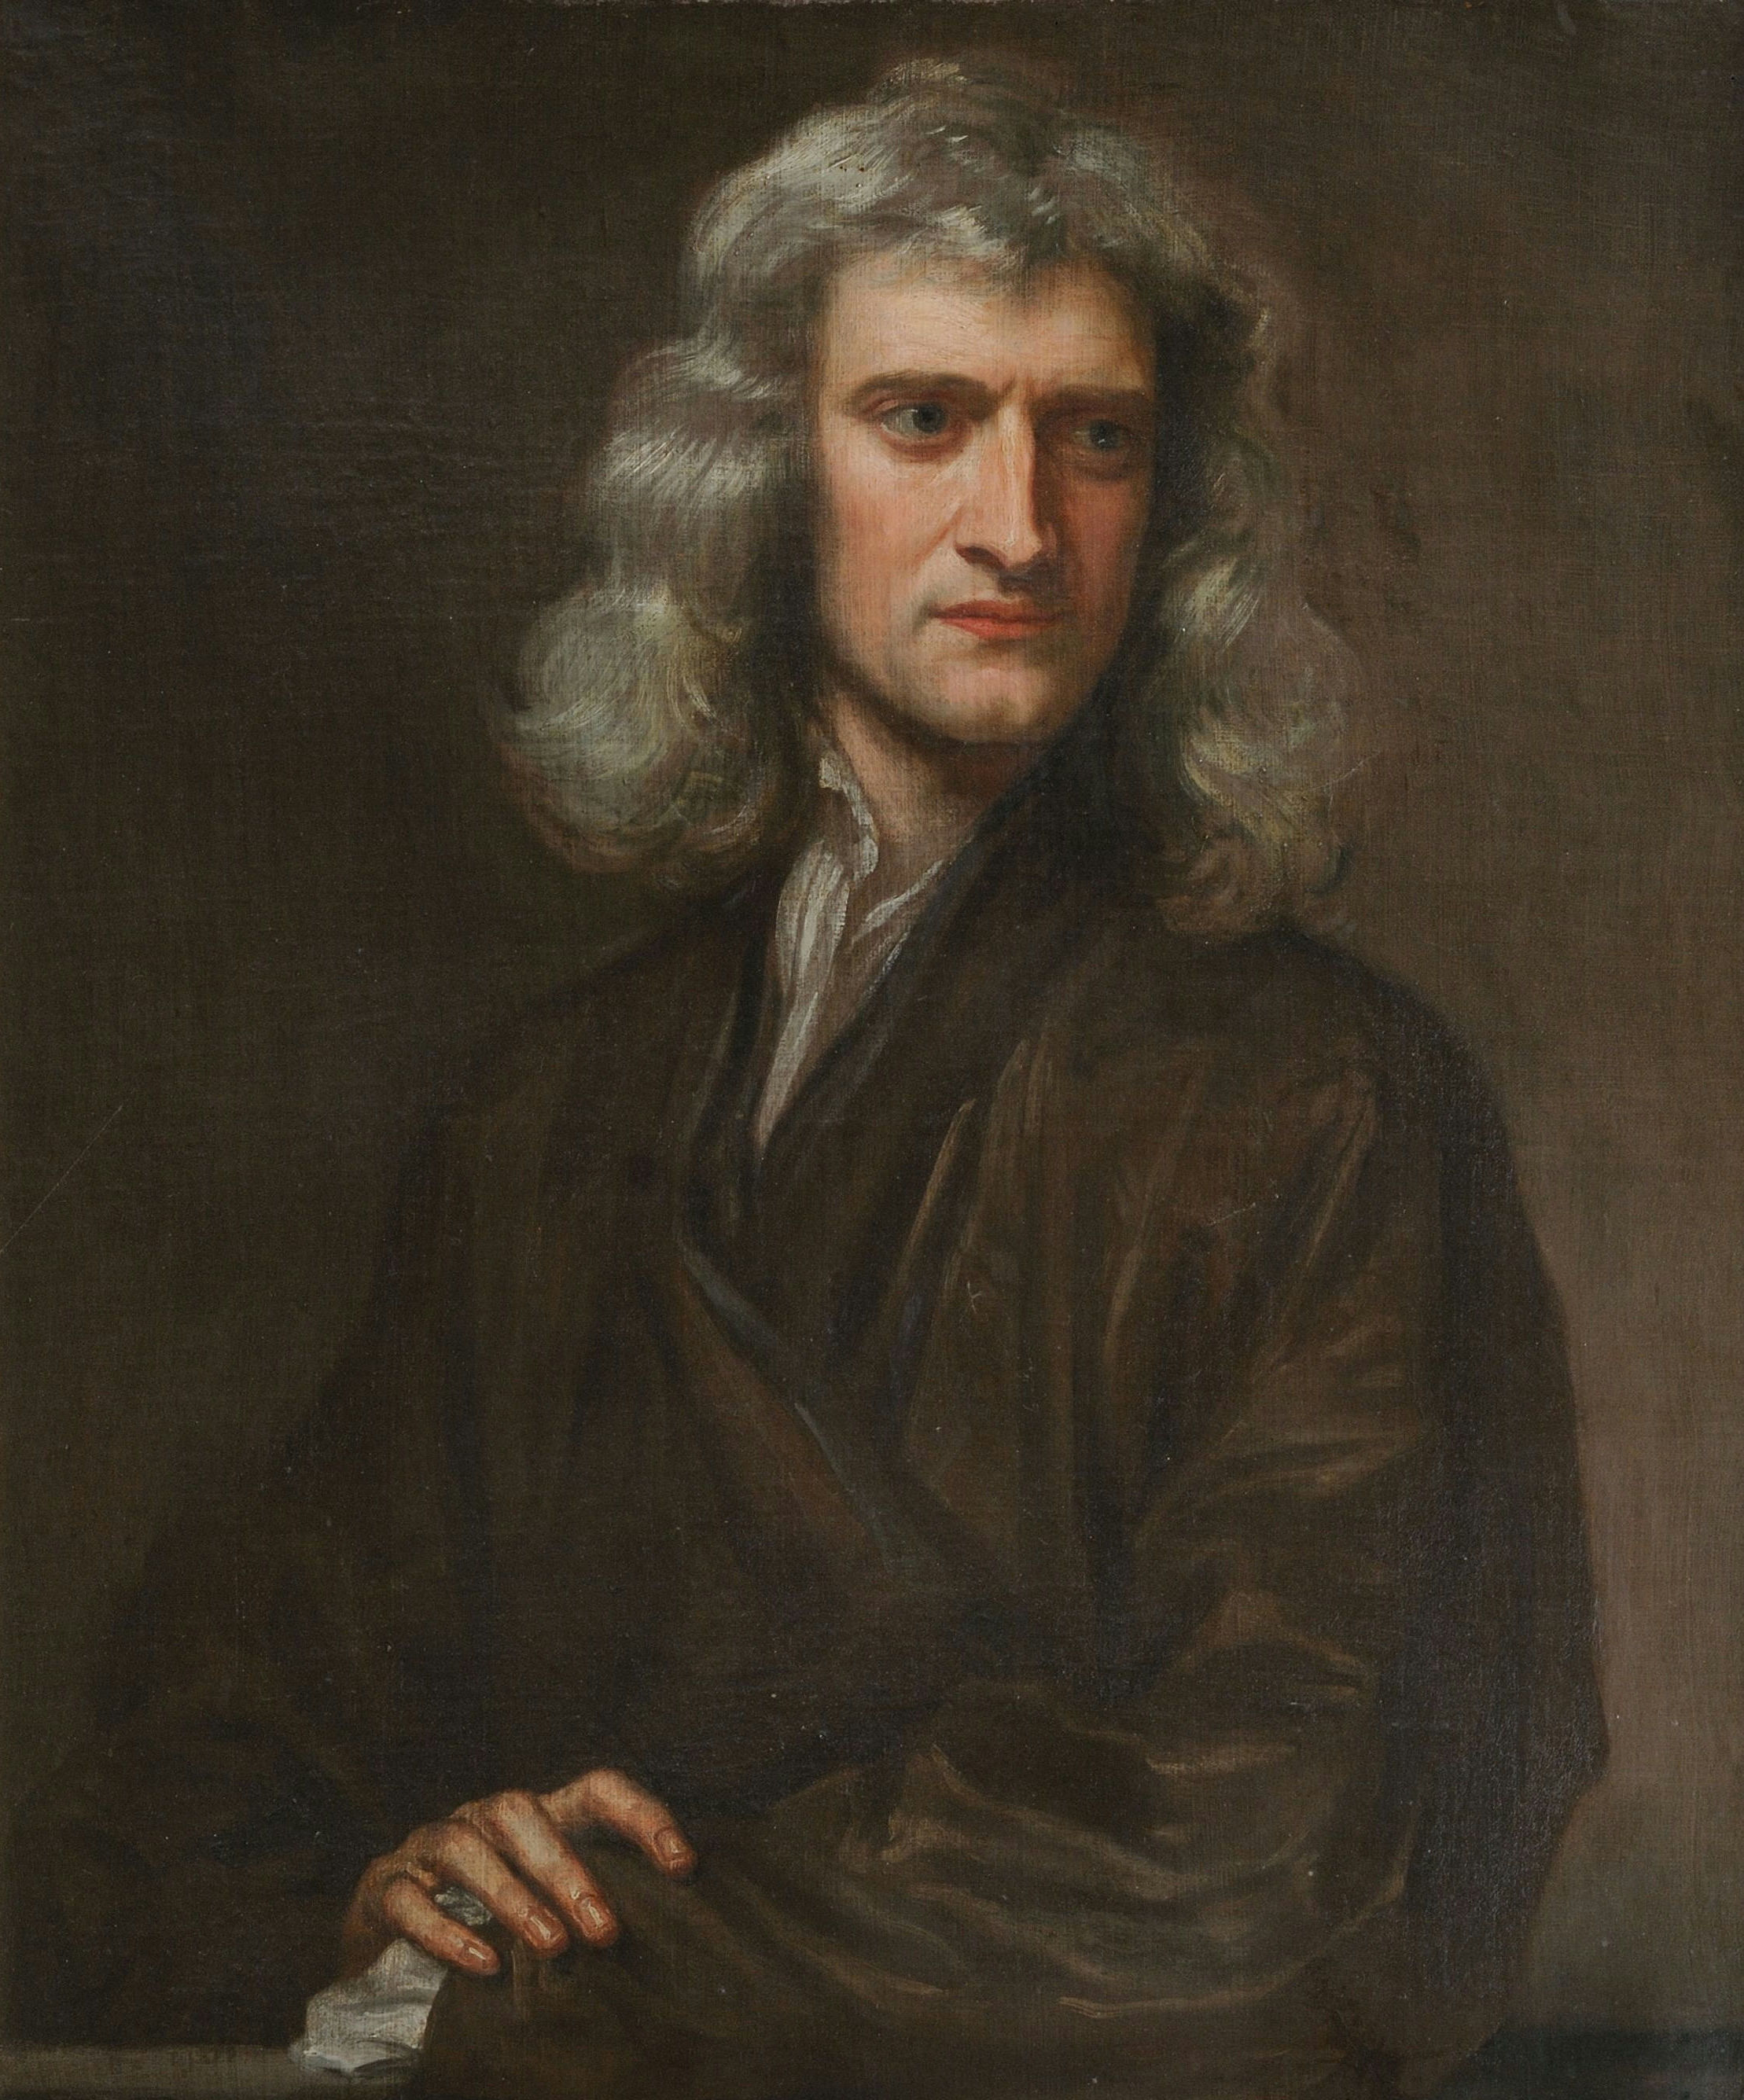
\includegraphics[width=0.4\textwidth]{figures/Portrait_of_Sir_Isaac_Newton,_1689.jpg}
    %}{A picture of the British mathematician and physicist Isaac Newton from Wikimedia commons.}
    \caption{A picture of the British mathematician and physicist Isaac Newton from \href{https://commons.wikimedia.org/wiki/File:Portrait_of_Sir_Isaac_Newton,_1689.jpg}{Wikimedia Commons}.}
\end{figure}

\paragraph{Newton's First Law:} The first law states that a body acted on by \textbf{no} net force moves with constant velocity (which may be zero) and zero acceleration. \\

This is the law that some find counter-intuitive since in everyday experience a ball rolling across a table will not keep rolling forever. However, in this situation there are net forces acting on the ball. There will be friction on the table and air resistance both acting to slow it down.\\

In the absence of friction or drag forces, motion really does persist until a force acts on an object. Think of an air hockey game, you apply an initial force to get the puck moving but after that it keeps travelling at a constant speed until it encounters another force, from the side of the table or the other players paddle. When friction is small we do see behaviour approximating Newton's first law, think of a person on roller skates or in a hover craft.

\paragraph{Newton's Second Law:} If a net external force acts on a body, the body accelerates. The direction of acceleration is the same as the direction of the net force. The mass of the body times its acceleration equals the net force.\\

This statement can look confusing but it is essentially saying that forces cause objects to accelerate and this is described mathematically by
\begin{equation}
\vec{F}_{\text{net}}=m\vec{a}.
\label{eq: N2}
\end{equation}

This is one of the most famous equations in physics and is commonly just referred to as Newton's second law. This equation is how we define the unit of force the Newton, with $1 \text{N}=1\text{kg m/s}^{2}$.  Note that $m\vec{a}$ is not necessarily a force itself, but is the vector sum of all the forces acting on an object. In many of the specific cases that we meet in this module, $F$ will just be one force.

\paragraph{Example 4.3:} Consider a vehicle of mass $600\text{kg}$ accelerating uniformly from rest to a velocity of $8.0\text{m/s}$ in $20$s. Find the force that needs to be applied to achieve this.\\

Recall that the first kinematic equation states that:
\begin{equation*}
a=\frac{v-u}{t}=\frac{8-0}{20}=0.4\text{m/s},
\end{equation*}
thus the force is
\begin{equation*}
F=ma=600\times 0.4=240\text{N}.
\end{equation*}

Newton's second law relies on knowing the mass of the object, but not which mass this is. There are two different definitions of mass in physics, the first is the \textbf{inertial mass}, defined through \cref{eq: N2}, which relates to how ``difficult'' it is to get an object moving. The second definition of mass is the \textbf{gravitational mass} which governs the strength of the gravitational force acting on an object. To the best of our ability to compare these different definitions of mass they agree.\\

What about weight? In everyday usage we use mass and weight interchangeably. However, in physics they are fundamentally different quantities. Mass is an intrinsic property of an object and a scalar quantity, while weight is the force of gravity acting on an object and is a vector. In other words, if the only force acting on an object is gravity, then the acceleration is $a=g$ and Newton's second law says that $mg=F_{W}=W$ is the weight of an object. Sometimes $g$ is referred to as the \textbf{gravitational field strength} as it is not actually constant, it decreases as your height above sea level increases.  The gravitational field strength will also be different on the moon or on a different planet, for example on the moon $g_{\text{moon}}=1.62\text{m/s}^{2}$.

\paragraph{Example 4.4:} Find the constant force needed to accelerate a $200\text{kg}$ mass to $6\text{m/s}$ in $4\text{s}$, neglecting air resistance.\\

First compute the average acceleration through:
\begin{equation*}
a=\frac{v-u}{t}=\frac{6-0}{4}=1.5\text{m/s}^{2},
\end{equation*}
then apply Newton's second law to find
\begin{equation*}
F=ma=200\times 1.5 =300\text{N}.
\end{equation*}

This is just considering the horizontal part of the motion, what about the vertical part? If we drew a free body diagram the vertical forces would be the wight pointing downward and a \textbf{normal reaction} force pointing upwards. The normal force is the support force of the ground acting on the object and stopping the object from falling through the ground. The weight and the normal force must be balanced if the object is not rising and falling. This opens up a new question, what is the normal force? This is where Newton's third law comes in.

\paragraph{Newton's Third Law:} If a body A exerts a force on body $B$ (an \textbf{action}), then body B exerts a force on body A (a \textbf{reaction}). These two forces have the same magnitude but opposite direction. These two forces act on \textbf{different} bodies.\\

Written as an equation this says that
\begin{equation*}
\vec{F}_{\text{A on B}}=-\vec{F}_{\text{B on A}}.
\end{equation*}
Often Newton's third law is expressed as ``Every action has an equal and opposite reaction''.

\paragraph{Example 4.5:} Consider a stationary ball on a table. The net force on the ball is zero since it is stationary and not accelerating. However, there is a \textbf{downward} force on the table from the ball, the weight of the ball. Newton's third law states that the table exerts an \textbf{upwards} force on the ball.\\

Newton's third law applies beyond contact forces, if we drop an apple then both the apple and the Earth accelerate towards each other. This explains the extra support or normal force that is always drawn on free body diagrams, it is the reaction force.\\


\section{Momentum and Collisions}
A closely related concept to force is \textbf{momentum}. It is a vector quantity denoted by $\vec{p}$ and given by the mass times the velocity. As an equation this is given by:
\begin{equation*}
\vec{p}=m\vec{v}.
\label{eq: momentum}
\end{equation*}

Momentum is a useful bookkeeping tool for studying objects in motion because in the absence of external forces the momentum is \textbf{conserved}. This makes it useful in analysing \textbf{collisions} between objects. In practice it is often easier to understand the effects of forces by applying conservation of momentum than by using Newton's second law. There is another conserved quantity that we will use to study motion, the \textbf{energy}. However, mechanical energy is \textbf{not always conserved}, while momentum is. e.g. when we study the collision between two cars, or a meteorite colliding with a planet, momentum is more convenient to use.\\

Momentum is measured in units of $\text{kg m/s}$ as defined through \cref{eq: momentum}.  We can rewritten Newton's second law in terms of the momentum to state that `` The rate of change of the momentum of an object is proportional to the resultant force on it.''

\paragraph{Example 4.6:} Consider an object of mass $m$ travelling at velocity $u$ before being acted on by a constant force $F$ and accelerating to velocity $v$. The initial momentum, before the force acts, is
\begin{equation*}
p_{i}=mu,
\end{equation*}
while the final momentum is 
\begin{equation*}
p_{f}=mv.
\end{equation*}
The change in momentum is thus
\begin{equation*}
\Delta p=p_{f}-p_{i}=mv-mu,
\end{equation*}
this will be positive if the object accelerates and negative if the object decelerates. Using Newton's second law we then get
\begin{equation*}
F=ma=m\frac{v-u}{t}=\frac{mv-mu}{t}=\frac{\Delta p}{t}.
\end{equation*}
This is a convenient rewriting of Newton's second law where $F$ is the force acting the object, $t$ is the length of time that the force is acting for, and $\Delta p$ is the change of momentum due to the force.

In general we will write the change of momentum as either $\Delta p$ or $\Delta \left(mv\right)$. The change in momentum is often referred to as the \textbf{impulse} and we saw above that it is given by the force multiplied by the time that the force acts over, $J=F t$. The example that we gave above had $m$ kept constant, however the mass can also change. This means that we should really write Newton's second law as
\begin{equation*}
F=\frac{\Delta\left(mv\right)}{\Delta t}.
\end{equation*}

If the mass changes at a constant rate but the velocity is constant then the force is 
\begin{align*}
F=v\frac{\Delta m}{\Delta t},
\end{align*}
that is the force depends on the change of mass per second.

\paragraph{Example 4.7:} The case of changing mass is important when studying rockets. A rocket ejects its burnt fuel at a constant speed. Then $v$ is the speed that the hot gas is expelled from the engine and $\Delta m/\Delta t$ is the mass of hot gas lost per second.  A nice discussion of the physics of the rocket equation is given in this \href{https://www.youtube.com/watch?v=V_brZ-KWY3g}{YouTube} video. Though be careful as a different sign convention is in the YouTube video.

\paragraph{Example 4.8:} Consider an object of mass $50 \text{kg}$ which is initially at rest before being acted on by a $10\text{N}$ force for $20\text{s}$. Find:
\begin{itemize}
\setlength{\itemsep}{-5pt}
    \item[a)] The change in momentum
    \item[b)] The velocity of the object after the force has acted.
\end{itemize} 

a) We know that 
\begin{align*}
F&=\frac{\Delta p}{\Delta t}\\
\Rightarrow \Delta p&=F\Delta t\\
&=10\times 20 =200 \text{Ns}.
\end{align*}

b) Now we now that the initial momentum is $p_{i}=0\text{kgm/s}$ and that at $20\text{s}$ the final momentum is $p_{f}=200\text{kgm/s}$. The velocity is thus
\begin{equation*}
v=\frac{p}{m}=\frac{200}{50}=4\text{m/s}.
\end{equation*}

From our everyday experience, we know that the harder we hit a ball the further it will travel. The impact changes the momentum over a very short time. We call the force associated with the change in momentum an \textbf{impact force},
\begin{equation*}
F=\frac{\Delta\left(mv\right)}{t}.
\end{equation*}

\paragraph{Example 4.9:} Consider a ball of mass $m=0.63\text{kg}$, initially at rest, which is struck by a bat and accelerated to a velocity of $35\text{m/s}$. The  contact time between the ball and the bat is $25\text{ms}$. Find:
\begin{itemize}
\setlength{\itemsep}{-5pt}
    \item[a)] The momentum gained by the ball.
    \item[b)] The average force acting on the ball.
\end{itemize} 
As in kinematics problem we start by writing down what we know and do not know about the initial and final configuration:
\begin{itemize}
\setlength{\itemsep}{-5pt}
    \item Initial:
    \begin{itemize}
\setlength{\itemsep}{-5pt}
    \item $t=0\text{s}$
    \item $u=0\text{m/s}$
    \item $p_{i}=mu=0\text{kgm/s}$
\end{itemize} 
    \item Final:
    \begin{itemize}
\setlength{\itemsep}{-5pt}
    \item $t=25\text{ms}$
    \item $v=35\text{m/s}$
    \item $p_{f}=?$
\end{itemize} 
\end{itemize} 
a) Calculate the change in momentum by finding the final momentum
\begin{equation*}
p_{f}=mv=0.63\times 35 =22\text{kgm/s}.
\end{equation*}

b) The impact force is
\begin{equation*}
F=\frac{\Delta p}{t}=\frac{22}{0.025}=880\text{N}.
\end{equation*}


Often it can be useful to plot force against time for an impact force. Typically we will find that the force acts over a very short time and can be quite sharply peaked. The average force of impact is the area under this curve.\\

\vspace{2cm}

\section{Impact and Conservation of Momentum}
Recall that momentum us a vector so when a ball bounces off a wall and rebound its momentum will change direction.  This is shown in \cref{fig: recoiling ball}. After a normal collision the ball rebounds and the direction of momentum is reversed. If we calculate $\Delta p$ we find that
\begin{equation*}
\Delta p=m(-u)-mu=-2mu,
\end{equation*}
this is with the sign convention that towards the wall is positive and away from the wall is negative.

\begin{figure}[ht]
    \centering
    \ThisAltText{A ball bouncing off a wall and reflected backwards with the velocity flipping its sign..}
    %\pdftooltip{
    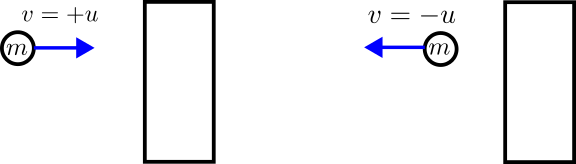
\includegraphics[width=0.4\textwidth]{figures/recoil.png}
    %}{A ball recoiling off a wall}
    \caption{A ball recoiling off a wall, the velocity afterwards is the negative of the velocity before.}
    \label{fig: recoiling ball}
\end{figure}

For an oblique impact we need to take account of the angle of incidence of the object on the wall -- done properly factors of $\cos\theta$ will show up when we work out what the initial and final momentum are. What we need to know is that the angle the ball comes in at will be equal to the angle it comes out at.

\paragraph{Example 4.10:} A tennis ball of mass $0.2\text{kg}$ moving at a speed of $18\text{m/s}$ is hit by a racket causing it to go back in the direction that it came from at a speed of $15\text{m/s}$. Given that the contact time is $0.12\text{s}$ find:
\begin{itemize}
\setlength{\itemsep}{-5pt}
    \item[a)] The change in momentum of the ball.
    \item[b)] The impact force on the ball.
\end{itemize} 
a) We know that $m=0.2\text{kg}$, $u=+18\text{m/s}$, and $v=-15\text{m/s}$, so 
\begin{equation*}
\Delta p=mv-mu=0.2\times(-15)-0.2\times 18=-6.6\text{kgm/s}.
\end{equation*}

b) Impact force is
\begin{equation*}
F=\frac{\Delta}{t}=-\frac{6.6}{0.12}=-55\text{N}.
\end{equation*}

An important principle when analysing impact forces and collisions is the \textbf{conservation of momentum}. This states that ``for a system of interacting objects, the total momentum remains constant provided no external resultant force acts on the system.''\\

Consider two objects which collide with each other then separate. The momentum of each object changes, but they exert equal and opposite forces on each other, by Newton's third law, so the total momentum is unchanged. In other words, the change in momentum of one object is equal and opposite to the change in momentum of the other object. \\

To see this in action consider two billiard balls $A$ and $B$ which collide and then separate. The impact force from $B$ on $A$ changes the velocity of $A$ from $u_{A}$ to $v_{A}$ in the contact time $t$. This force is
\begin{equation*}
F_{1}=\frac{m_{A}v_{A}-m_{A}u_{A}}{t},
\end{equation*}
by analogy
\begin{equation*}
F_{2}=\frac{m_{B}v_{B}-m_{B}u_{B}}{t}.
\end{equation*}

From Newton's third law these forces are equal and opposite so $F_{1}=-F_{2}$, which means that
\begin{equation*}
\frac{m_{A}v_{A}-m_{A}u_{A}}{t}=-\frac{m_{B}v_{B}-m_{B}u_{B}}{t},
\end{equation*}
which rearranges to

\begin{equation*}
m_{A}u_{A}+m_{B}u_{B}=m_{A}v_{A}+m_{B}v_{B}.
\end{equation*}

We often write this as in terms of the momentum as
\begin{equation}
p_{i}=p_{f}
\label{eq: conservation of momentum}
\end{equation}

\paragraph{Example 4.11:} A wagon $A$ of mass $4500\text{kg}$ is moving along a level track at a speed of $3\text{m/s}$ when it collides with and couples to a second wagon $B$ of mass $3000\text{kg}$ which is initially stationary. Calculate the velocity of the two wagons after the collision.\\

Note that since the objects stick together after the collision, the conservation of momentum becomes
\begin{equation*}
m_{A}u_{A}+m_{B}u_{B}=(m_{A}+m_{B})v_{f}.
\end{equation*}

The initial momentum is
\begin{equation*}
p_{i}=m_{A}u_{A}+m_{B}u_{B}=4500\times 3+3000\times 0=13500\text{kgm/s}.
\end{equation*}
The final momentum is
\begin{equation*}
p_{f}=v_{f}(4500+3000) \text{kg} =v_{f}\times 7500\text{kg}.
\end{equation*}
Conservation of momentum then implies that
\begin{align*}
v_{f}\times 7500\text{kg}&=13500\text{kgm/s}\\
v_{f}&=\frac{13500}{7500}\text{m/s}=1.8\text{m/s}.
\end{align*}

In the next section we will meet another quantity that we can also use to study objects in motion, and more generally. The \textbf{energy}.  While momentum is always conserved, in the absence of net external forces, mechanical energy is not. This leads us to distinguish between two different types of collisions: \textbf{elastic collisions} where both are conserved, and \textbf{inelastic collisions} where momentum is conserved but mechanical energy is not. Here \textbf{mechanical energy} means the kinetic energy or energy of motion. You can practice using the conservation of momentum by solving some of the problems on the tutorial sheet.